\section{Resultados}
\subsection{Princípio de Arquimedes}

% TODO: Magina, coloque apenas os resultados e os erros das medidas (apenas das
% medidas)

\subsection{Balança de empuxo}

Os dados coletados foram sintetizados na \cref{tab1} junto aos valores
disponibilizados na ficha técnica dos aparelhos.
\begin{table}[H]
    \caption{Resultados da balança de empuxo e valores de referência}
    \label{tab1}
    \begin{center}
        \begin{tabular}{c c c}
            \hline
            Item & Peso medido & Valor de referência\\
            \hline
            Peso redondo & \( (510 \pm 25) \unit{\gram} \) & \( - \) \\
            HD & \( (640 \pm 25) \unit{\gram} \) & \( - \) \\
            Celular Q. & \( (270 \pm 25) \unit{\gram} \) & \( 308 \unit{\gram} \) \\
            Celular B. & \( (250 \pm 25) \unit{\gram} \) & \( 204 \unit{\gram} \) \\
            Celular M & \( (200 \pm 25) \unit{\gram} \) & \( 169 \unit{\gram} \) \\
            Celular J. & \( (170 \pm 25) \unit{\gram} \) & \( 169 \unit{\gram} \) \\
            Celular L. & \( (220 \pm 25) \unit{\gram} \) & \( 177 \unit{\gram} \) \\
            \hline
    \end{tabular}
    \end{center}
\end{table}

\subsection{Gangorra}

% TODO: Coloque aqui

\subsection{Bonecos flutuantes}

Todos os integrantes do grupo foram capazes de realizar o desafio proposto, veja
a \cref{figdesafio}. Além disso, observou-se que, ao pressionar a garrafa, o
boneco submergia, retornando à posição flutuante quando a pressão era liberada.
O movimento do boneco ocorria de maneira consistente, independentemente do local
onde a garrafa era apertada, sugerindo uma relação direta com a variação de
pressão no interior do recipiente. O fenômeno se repetiu de forma idêntica em
todas as tentativas realizadas.

\begin{figure}[H]
    \centering
    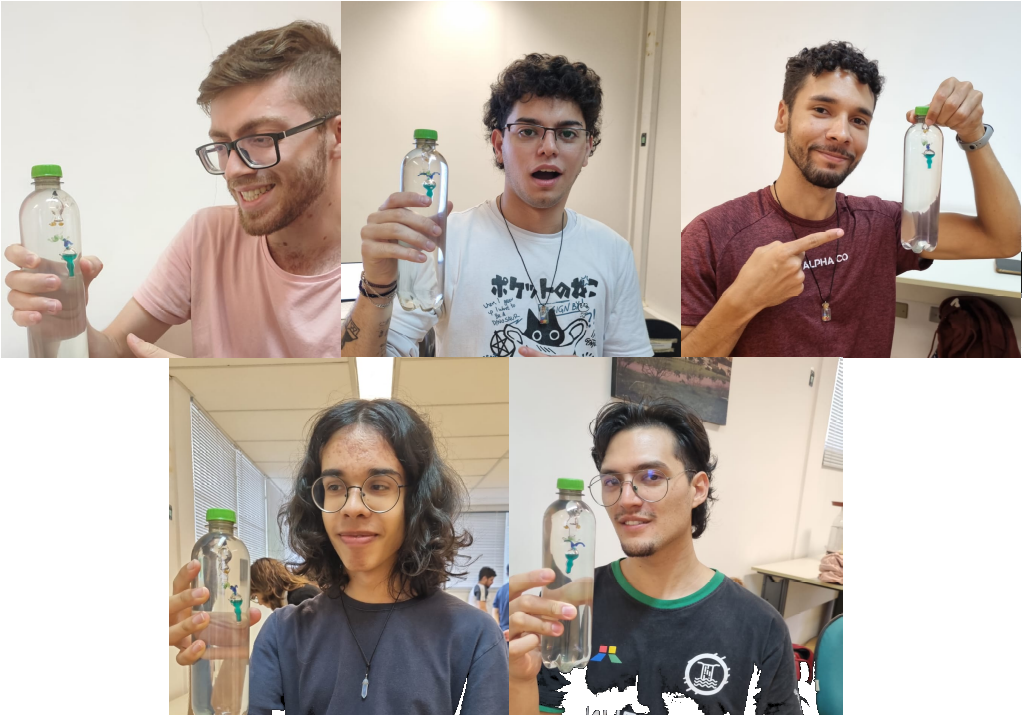
\includegraphics[width=.5\linewidth]{fig/desafio.png}
    \caption{Integrantes do grupo sorrindo após concluírem o desafio}
    \label{figdesafio}
\end{figure}


